\documentclass[10pt,a4paper]{article}
\usepackage[utf8]{inputenc}
\usepackage{polski}
\usepackage{amsmath}
\usepackage{amsfonts}
\usepackage{amssymb}
\usepackage{graphicx}
\usepackage{verbatim}
\usepackage{minted}
\usepackage{amsmath}
\usepackage{algorithm}
\usepackage[noend]{algpseudocode}
\usepackage{csvsimple}
\usepackage{caption}
\usepackage{subcaption}
\usepackage{hyperref}
\usepackage{url}



\author{Onaszkiewicz Przemysław, Gadawski Łukasz}
\title{Temat 2\\ Dla wskazanego kandydata w wyborach w USA, przedstaw w sposób czytelny na mapie finansowanie jego kampanii wyborczej, z uwzględnieniem darowizn bezpośrednich i poprzez komitety wyborcze. 
}

\begin{document}
\maketitle

\section{Funkcjonalności}
\begin{enumerate}
\item Wybór rocznika wyborów prezydenckich  
Użytkownik będzie miał możliwość wybrania dane z których wyborów chce oglądać. Dostępne będą tylko dane z wyborów prezydenckich.
\item Wybór kandydata z listy. W systemie będzie dostępna lista kandydatów którzy brali udział w wyborach. Użytkownik będzie miał możliwość wybrania konkretnego kandydata i wyświetlenia danych o dotacjach dotyczących tylko jego kandydatury. Będzie też możliwość wyświetlenia zagregowanych danych dotyczących wszystkich kandydatów. 
\item Wybór prezentowanych danych na mapce:
\begin{enumerate}
\item wielkość wszystkich środków uzyskanych z danego regionu 
\item wielkość darowizn bezpośrednich
\item wielkość dotacji od komitetu wyborczego 
\end{enumerate}
 Będzie to dodatkowa możliwość. Po jej wybraniu nastąpi dodatkowe filtrowanie danych pod kątem regionu w którym wpłynęły, jak również rodzaju darowizn (bezpośrednie i od komitetów “POC”).
\item Wybór prezentacji danych na mapie:
\begin{enumerate}
\item dla całego kraju
\item poszczególnych stanów
\item ewentualnie rejon danego kodu pocztowego
\end{enumerate}

W początkowej fazie dane będą pokazane na obszarze całego kraju. Po wejściu w 
konkretny  stan zostaną wyświetlone bardziej szczegółowae dane na jego temat 
(podział na mniejsze okręgi). 

\end{enumerate}
\section{Pobranie danych dotyczących wyborów}
Do pobrania danych dotyczących wyborów rozpatrywaliśmy API jakie udostępnia New York Times na swoich stronach. Dane można uzyskać w formacie xml w formacie json.   
Rozpatrywano dwa sposoby pobierania danych. Pierwszym z nich było korzystanie z API wystawionego przez New York Times  do pobierania danych w formacie json. Kolejnym było pobranie na dysk plików z danymi dotyczącymi wyborów bezpośrednio na dysk twardy i przechowywanie ich w bazie danych.
\subsection{New York Times API- pobieranie potrzebnych fragmentów danych w formacie json}
\textbf{Indywidualne wpłaty na danego kandydata:}

Zapytanie \cite{derekwillis2015ind} pozwala na pobranie danych o indywidualnych darczyńcach. Z uwzględnieniem ich miejsca zamieszkania. Filtrując dane można uzyskać dane o wysokości darowizn od darczyńców indywidualnych  z danego regionu geograficznego,  jak również o ilości wpłat na danego kandydata w danym regionie.
\\
\\
\textbf{Finansowanie kandydata przez komitet z danego dystryktu stanu:}

Zapytanie \cite{derekwillis2015com} pozwala uzyskać wysokość wpłat przekazanych na rzecz danego kandydata w danym dystrykcie wyborczym. Pozwala to uzyskać dane o wysokości wpłat komitetów na rzecz kandydata(i ich procentowego udziału w totalnej kwocie zebranej przez niego ).

\subsection{Pobranie plików zawierających dane o finansach bezpośrednio ze stron FEC}

Drugim rozpatrywanym sposobem uzyskania danych na temat finansowania kampanii kandydatów w wyborach prezydenckich jest pobieranie danych do kampanii bezpośrednio ze stron FEC i załadowanie ich do bazy danych.
Poniżej przedstawiono opis zawartości poszczególnych plików w celu przedstawienia jakie dane można za ich pomocą uzyskać.

\begin{itemize}
\item Plik zawierający dane na temat wpływów do kandydatów od komitetów. \cite{fecContToCandFromComit}
\begin{itemize}
\item Candidate Identification Number
\item Filer Identification Number (CMTE\_ID)
\item Zip Code
\item State
\item City/Town
\item Transaction Amount
\item Transaction ID
\item Entity Type
\begin{itemize}
\item CAN = Candidate
\item CCM = Candidate Committee
\item COM = Committee
\item IND = Individual (a person)
\item ORG = Organization (not a committee and not a person)
\item PAC = Political Action Committee
\item PTY = Party Organization)
\end{itemize}
\end{itemize}

\item Plik zawierający dane na temat wpływów do komitetów z indywidualnych dotacji.
\cite{fecIndividualContributionMasterFileDescriptionSite2015}

\begin{itemize}
\item Filer Identification Number (CMTE\_ID)
\item Zip Code
\item State
\item City/Town
\item Transaction Amount
\item Transaction ID
\item Entity Type 
\end{itemize}

\item Plik zawierający złączenie kandydat - komitet którego bardziej szczegółowy opis znajduje się na stronie \cite{fecCandidateComiteeLinkageFile2015} 


\begin{itemize}
\item Committee Identification (CMTE\_ID)
\item Committee Name
\item Zip Code
\item State
\item City or Town
\end{itemize}


\item Plik zawierający dane na temat kandydatów i ich szczegółowy opis \cite{fecCandMasterFile2015}.

\begin{itemize}
\item Candidate Identification
\item Candidate Name
\item Candidate Office
\begin{itemize}
\item H = House
\item P = President
\item S = Seante
\end{itemize}
\item Year of Election
\item Candidate State
\item Candidate District
\end{itemize}


\item Plik zawierający komitety którego opis znajduje się pod adresem \cite{fecComMasterFile2015}.

\begin{itemize}
\item Committee Identification (CMTE\_ID)
\item Committee Name
\item Zip Code
\item State
\item City or Town
\end{itemize}
\end{itemize}


Dane pochodzące ze strony FEC dane dotyczące finansowania są przechowywane w plikach tekstowych o przedstawionej powyżej strukturze. Na potrzeby naszej aplikacji powstanie narzędzie parsujące te pliki tekstowe oraz przeprowadzające ich zapis do bazy danych o analogicznej strukturze tabel. 
\section{pobranie danych geograficznych}
Dane geograficzne można pobrać w dwóch formach. Jedn z nich jes formą punktową a druga obszarową.
\subsection{Punktowe dane o ZIP kodach\label{sec:punktZIP}}
Dane o ZIP kodach można pobrtać w postaci plików z rozszerzeniem CSV. Zawierają one dane takie jak ZIP, latitude(długość) i longtitude(szerokość).

Sprawia to że zip kody są na umiejscowione na mapie, ale ich występowanie jast punktowe.
Być może na potrzeby projektu taka reprezentacja była by wystarczająca. dane dotyczące finansowania wyborów na danym obszarze przedstawiano by za pomocą słupków w tych punktach.

\subsection{Obszarowe dane o ZIP kodach\label{sec:obszZIP}}
Dane geograficzne można odnaleźć w kilku miejscach.
Między innymi jest to otwarty plik Catrographic Shapefile pochodzący ze strony \cite[US Census Bureau]{unitedStateCensusBureauGeoMaps}
i zawierający około 33143 kodów.

\begin{figure}[H]
    \centering
    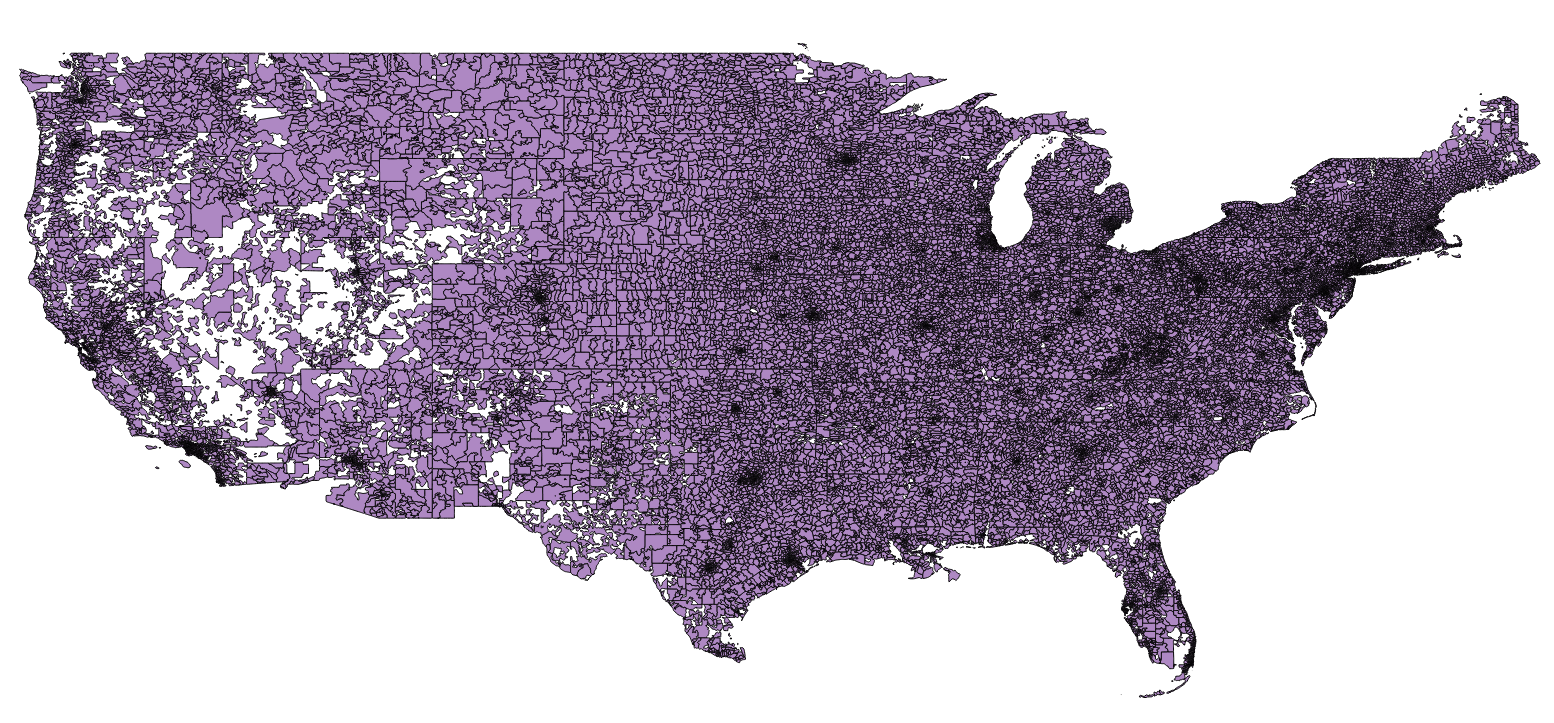
\includegraphics[width=0.8\textwidth]{bazaUSCB.png}
    \caption{Rysunek przedstawiający pokrycie kodów pocztowych z bazy USCB na obszarze USA}
    \label{fig:imageUSCB}
\end{figure}

Kolejną bazą ZIP kodów jest baza kodów ESRI dostępna pod adresem \cite[Arcgis]{arcgisDatabase} na stronie istnieje również opis jak można skonwertować dane do Shapefile'a. Kodów dostępnych w tej bazie jest około 30541. 

\begin{figure}[H]
    \centering
    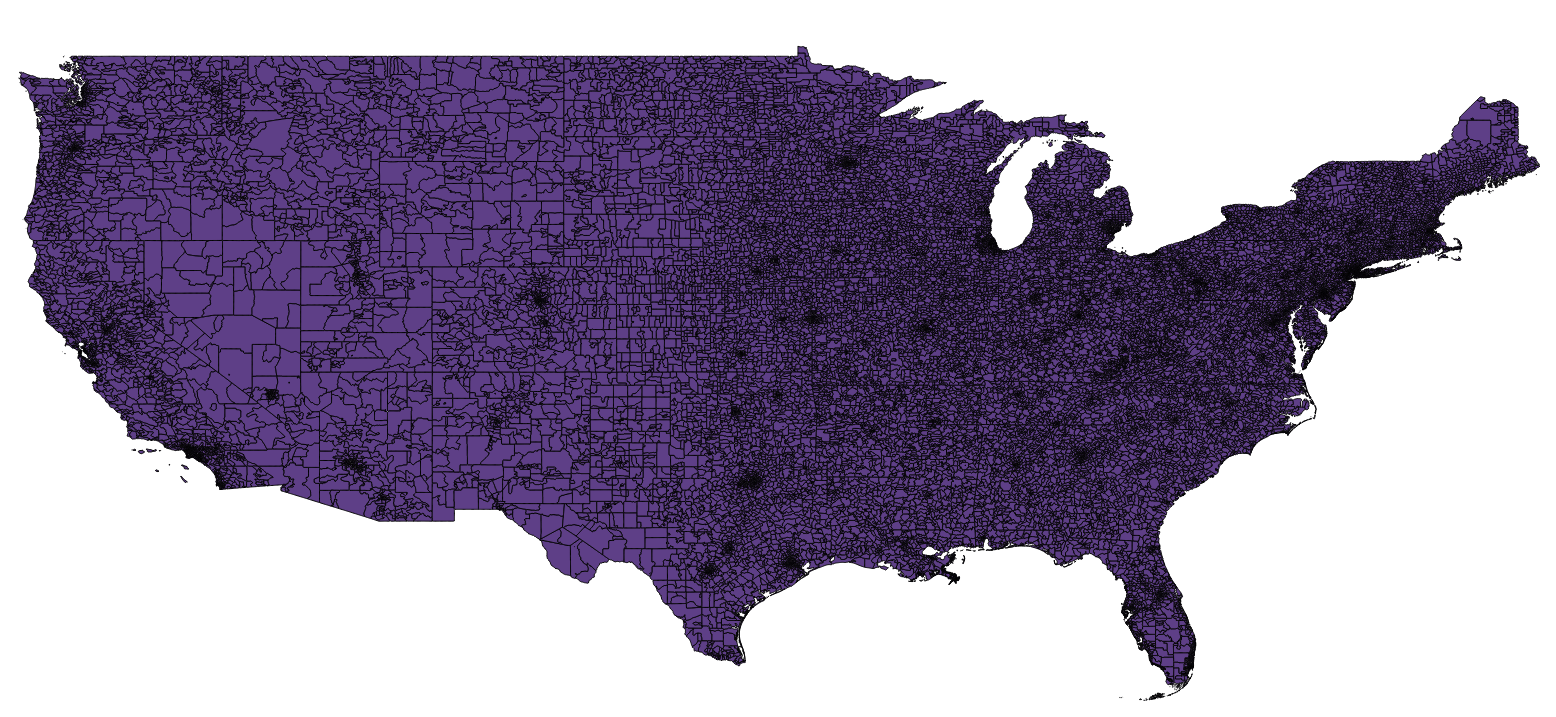
\includegraphics[width=0.8\textwidth]{bazaESRI.png}
    \caption{Rysunek przedstawiający pokrycie kodów pocztowych z bazy ESRI na obszarze USA}
    \label{fig:imageESRI}
\end{figure}
 
Wszystkich kodów w  USA jest około 42000, najwięcej zawiera baza  \textit{U.S. Census Bureau} przytoczona powyżej (33143) i podaje przybliżone regiony, natomiast dane pobrane ze strony firmy ESRI zawierają 30541 rekordów. Pomimo to przy wizualizacji obu warstw okazuje się, że dane od firmy ESRI mają lepszą dokładność i większe pokrycie USA. Może to być spowodowane tym że dane z US CB posiadają zduplikowane dane bądź regiony na siebie zachodzą i występuje redundancja danych.


\subsection{Wybranie klucza złączenia}
Na podstawie danych dostarczonych przez FEC kluczem złączenia danych dotyczących finansowania kampanii kandydatów mogą być następujące atrybuty zawierające dane geograficzne:

\begin{itemize}
\item Zip Code
\item State
\item City or Town
\end{itemize}

Dana dotycząca stanu może być na nasze potrzeby zbyt ogólna, podobnie informacja o mieście lub wsi, taki klucz może nie być wystarczająco precyzyjny, co więcej dane geograficzne zawierające takie dane mogą zawierać tylko wycinki obszarów. Najbardziej dokładnym atrybutem jest kod pocztowy. Należy mieć jednak na uwadze, że taka dana również nie jest idealną reprezentacją, ponieważ kod pocztowy w głównym zamyśle powstał dla ułatwienia organizacja przesyłek pocztowych, dlatego też często zdarza się, że wieżowiec lub wielkie przedsiębiorstwo zajmujące spory obszar geograficzny może posiadać swój indywidualny kod pocztowy. 

Kody pocztowe mogą zostać przedstawione w dwojakiej formie. Pierwszą jest wizualizacja danych na podstawie punktowych danych dotyczących kodów pocztowych. Tzn. każdy kod pocztowy posiada współrzędne geograficzne do niego przypisane. Znalezione dane punktowe są najdokładniejsze, ponieważ zawierają współrzędne dla 42522 kodów i można wnioskować, że są to wszystkie występujące dane. Problemem w przypadku ewentualnej wizualizacji naszego problemu finansowania kampanii wyborczej może być sposób prezentacji na mapie takich danych. Można byłoby tego dokonać za pomocą różnej wielkości słupków, bądź okręgów przypisanych do danej długości i szerokości geograficznej. Niewątpliwą zaletą tej metody jest dokładność, ponieważ najprawdopodobniej wszystkie dane geograficzne uzyskałyby złączenie z danymi dotyczącymi finansowania.

Drugim sposobem są przybliżone obszary w postaci wielokątów na mapie obrazujących dany kod pocztowy. Pobrane dane geograficzne ze strony firmy ESRI po dokładnym przyjrzeniu się mapom wydają się być najbardziej precyzyjne i obejmować niemalże cały obszar USA, pomimo tego, że zawierają 30541 rekordów w stosunku do około 42000 wszystkich kodów pocztowych występujących w USA. Zaletą tego sposobu przedstawienia danych byłaby możliwość przedstawienia danych dotyczących finansowania poprzez gradient konkretnych obszarów. Wadą jest w tym przypadku potencjalna niedokładność prezentacji danych, lub wręcz brak prezentacji niektórych danych finansowych poprzez brak złączenia z danymi geograficznymi.

\section{Technologie wykonania}

Na potrzeby tworzonej aplikacji zostanie stworzona struktura przechowująca pobrane dane dotyczące finanosowania kandatów. Zostanie stworzony skrypt, który zapisze potrzebne dane z plików CSV do bazy danych \textit{\textbf{PostgreSQL}}. Dane geograficzne również będą przechowywane w bazie danych, dodatkowo będzie zainstalowana nakładka \textit{\textbf{PostGIS}} umożliwiająca wykonywanie zapytań przestrzennych.

Pobieranie danych o ZIP kodach było rozpatrywane w dwóch wariantach: punktowym (\ref*{sec:punktZIP}) i obszarowym (\ref*{sec:obszZIP}). Zdecydowano się na pobranie ich w formie obszarowej. Najprawdopodobniej będzie to lepiej służyło potrzebom aplikacji. Spośród dwóch rozpatrywanych baz (ESRI i USCB) lepsza wydaje się baza \textit{\textbf{ESRI}}. Ponieważ pomimo mniejszej ilości występujących w niej kodów, na rysunkach \ref{fig:imageESRI} i \ref{fig:imageUSCB} widać że baza \textit{\textbf{ESRI}} ma większe pokrycie na terenie całego USA. To pokrycie obszaru USA w połączeniu z danymi adresowymi darczyńcy będzie mogło posłużyć do złączenia danych nawet w przypadku nie występowania ZIP kodu darczyńcy w bazie.  

Z uwagi na chęć zapewnienia największej elastyczności w pobieraniu oraz prezentacji danych zostanie stworzona aplikacja internetowa umożliwiająca serwowania danych w przeglądarce. Do tego celu zostanie wykorzystany \textit{\textbf{Geoserver}}, czyli serwer aplikacyjny, który będzie odbierał przy pomocy REST API zapytań HTTP o zawartość do wyświetlenia. \textit{\textbf{Geoserver}} jako popularny kontener serwletów umożliwia w prosty sposób połączenia z bazą danych PostgreSQL oraz prezentację danych geograficznych.

Warstwa prezentacji, czyli stworzenie komponentów HTML umożliwiających opisane w pierwszym punkcie funkcjonalności (np. wybór wyborów oraz kandydatów), zostanie wykonana przy pomocy biblioteki języka JavaScript \textit{\textbf{AngularJS}}. Umożliwia on w prosty sposób konstruowanie żądań HTTP do danego API, a także pozwala jego zastosowanie pozwoli odseparować warstwę widoku od serwera aplikacji i danych. 


\section{Pomocne linki}
W niniejszej sekcji znajdują się linki do żródeł, na które autorzy natrafili podczas prób zdiagnozowania problemu.
\begin{itemize}
\item \cite[Atrykuł przedstawiający ładowanie ShapeFile do bazy danych PostGIS]{loadShpDataIntoPostGis}
\item \cite[Atrykuł pokazujący obsługę GeoSerwera]{servepostgisdata1}
\item \cite[Wątek opisujący załadowanie pliku z bazą danych eESRI i konwersje fo Shapefile'a]{loadESRIDataAndConvertToShape}
\item \cite[Strona Wiki opisująca sposób ekstrakcji danych geograficznych do bazy postGisowej]{osmToPostGIS}
\end{itemize}
\bibliography{bibliografia}{}
\bibliographystyle{plain}
\end{document}